\section{Introduction}%
\label{sec:introduction}

The aim of this thesis is to explore and hopefully gain some insight into the
nature of infinite neural networks kernels. These are a family of kernels
which are obtained analytically from the limit of infinite width of a neural network.
This section provides a brief introduction to the concepts and techniques from which
the kernels are derived.

\subsection{Neural networks}%
\label{sub:neural_networks}

In its most basic form, a neural network is a function which maps an input vector
$\textbf{x}$ to an output vector $\textbf{y}$. This function is defined by a set of
parameters $\textbf{w}$ which are learned from the training samples.

There are many architectures for neural networks, but we are going to focus
on the most basic one, a single hidden layer feedforward neural network. This is a
neural network with a single hidden layer of neurons (units) between the input and
the output layers. We can define the function $f$ of a single hidden layer feedforward
neural network as follows:

\begin{equation}
    f(\textbf{x},\,\textbf{w}) = \textbf{W}_2 \sigma \left( \textbf{W}_1 \textbf{x} + \textbf{b}_1 \right) + \textbf{b}_2
\end{equation}
where $\textbf{W}_1$ and $\textbf{W}_2$ are the weight matrices of the first and second layers respectively,
$\textbf{b}_1$ and $\textbf{b}_2$ are the bias vectors of the first and second layers respectively and
$\sigma$ is the activation function.

A diagram of such a neural network is shown in \cref{fig:neural_network}.

\begin{figure}[H]
    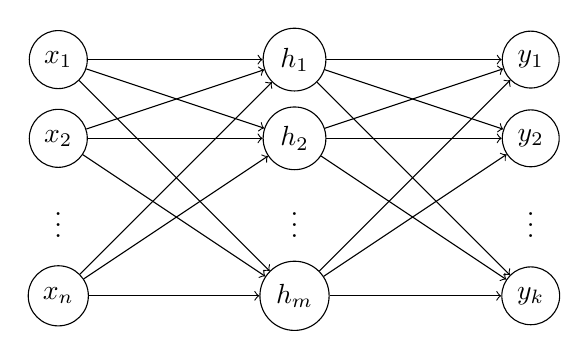
\begin{tikzpicture}
        % Input layer
        \node[draw, circle] (x1) at (0, 0) {$x_1$};
        \node[draw, circle] (x2) at (0, -1) {$x_2$};
        \node (x3) at (0, -2) {$\vdots$};
        \node[draw, circle] (x4) at (0, -3) {$x_n$};

        % Hidden layer
        \node[draw, circle] (h1) at (3, 0) {$h_1$};
        \node[draw, circle] (h2) at (3, -1) {$h_2$};
        \node (h3) at (3, -2) {$\vdots$};
        \node[draw, circle] (h4) at (3, -3) {$h_m$};

        % Output layer
        \node[draw, circle] (y1) at (6, 0) {$y_1$};
        \node[draw, circle] (y2) at (6, -1) {$y_2$};
        \node (y3) at (6, -2) {$\vdots$};
        \node[draw, circle] (y4) at (6, -3) {$y_k$};

        % Connections
        \foreach \i in {1,2,4} {
            \foreach \j in {1,2,4} {
                \draw[->] (x\i) -- (h\j);
                \draw[->] (h\i) -- (y\j);
            }
        }
    \end{tikzpicture}
    \caption{Diagram of a single hidden layer feedforward neural network.}%
    \label{fig:neural_network}
\end{figure}

Computation in \emph{infinite} neural networks was first explored by
\textcite{nealBayesianLearningNeural1996} in the context of Gaussian
processes by applying Bayesian inference to neural networks.

\subsection{Bayesian Neural Networks}%
\label{sub:bayesian_neural_networks}

From a statistical point of view, the standard approach to training
backpropagation neural networks using gradient descent to minimize the
loss function can be interpreted as
\emph{maximum likelihood estimation} (MLE) of the parameters of the model.
The training process is thus an optimization problem from which we obtain
the \emph{optimal} set of parameters given the data.

On the other hand, using Bayesian inference, the prediction obtained is based
on \emph{all} the possible values of the parameters, weighted by the corresponding
probability of each set of parameters (the posterior distribution). This means
that the prediction is not a single value, but a distribution of values. We are therefore
dealing with an \emph{integration problem}.

The main benefits of using the Bayesian approach is that it provides an
indication of the uncertainty of the prediction and that it reduces ``overfitting''.
However, the main drawback is that the integration is intractable for
complex models, such as neural networks and requires Markov Chain Monte Carlo
methods or other techniques to approximate the posterior distribution \cite{nealBayesianTrainingBackpropagation1992}.

\subsubsection{Bayesian neural network training problem}%
\label{ssub:bayesian_neural_network_training_problem}

Below is a summary of the formulation for the Bayesian neural network from \textcite{nealBayesianTrainingBackpropagation1992}.
The formulation if for the regression case, but it can be easily extended to the classification case.

Assuming we have a set of $n$ independent training samples,
$\left(\textbf{x}_1,  \textbf{y}_1 \right),\,\dots,\,\left(\textbf{x}_n,  \textbf{y}_n \right)$
each of which consists of an ``input'' vector $\textbf{x}_i$ associated to an ``output'' vector $\textbf{y}_i$.
And given an additional item $\textbf{x}_{n+1}$, we want to predict the corresponding $\textbf{y}_{n+1}$.

We define a neural network of an arbitrary architecture with a $\textbf{w}$ vector of parameters as a function
$f$ which maps an input vector $\textbf{x}$ to an output vector $\widehat{\textbf{y}}$. Formally: $\widehat{\textbf{y}} = f(\textbf{x},\,\textbf{w})$.

If we assume a Gaussian noise model, the conditional probability distribution for the output given the output is given by:
\begin{equation}
    P(\textbf{y} \mid \textbf{x},\,\textbf{w}) = \mathcal{N}(\textbf{y} \mid f(\textbf{x},\,\textbf{w}),\,\sigma^2)
    = \left(2\pi\sigma^2\right)^{-\frac{D}{2}} \exp \left( -\frac{1}{2\sigma^2} \left\lVert \textbf{y} - f(\textbf{x},\,\textbf{w}) \right\rVert^2 \right)
\end{equation}
where $D$ is the dimensionality of the output vector $\textbf{y}$ and $\sigma^2$ is the variance of the noise\footnote{
    This assumes a constant noise level, but extending it to a noise model with a different variance for each sample is straightforward.
}

The maximum likelihood approach consists of finding the parameters $\textbf{w}$ that maximize the likelihood of the training data
through a gradient descent algorithm. This can be formalized as the maximization of the log-likelihood $L(\textbf{w})$:
\begin{equation}%
    \label{eq:log_likelihood}
    L(\textbf{w}) = \sum_{i=1}^{n} \log P(\textbf{y}_i \mid \textbf{x}_i,\,\textbf{w})
\end{equation}

From the maximization of the log-likelihood, we obtain the optimal set of parameters $\widehat{\textbf{w}}$ and then use it
to predict the output $\widehat{\textbf{y}}_{n+1} = f(\textbf{x}_{n+1},\,\widehat{\textbf{w}})$.

In the Bayesian approach, instead of using a \emph{single} ``best'' set of weights, we integrate the predictions from all possible
weight vectors over the posterior weight distribution. This is equivalent to averaging the predictions of all possible neural networks
with different weights. The best single-value prediction for our new sample $\textbf{x}_{n+1}$ is then given by:
\begin{equation}\label{eq:bnn_single_prediction}
    \widehat{\textbf{y}}_{n+1} = \int_{\mathds{R}^N}
        f(\textbf{x}_{n+1},\,\textbf{w})
        P(\textbf{w} \mid \left(\textbf{x}_1,  \textbf{y}_1 \right),\,\dots,\,\left(\textbf{x}_n,  \textbf{y}_n \right))
        \,d\textbf{w}
\end{equation}
where $N$ is the dimensionality of the weight vector $\textbf{w}$.

The single value from \cref{eq:bnn_single_prediction} is the \emph{expected value} of the posterior distribution of the output given the input.
However, we are interested in the \emph{full} posterior distribution of the output given the input, which is given by:
\begin{multline}\label{eq:bnn_posterior}
    P(\textbf{y}_{n+1} \mid \textbf{x}_{n+1},\,\left(\textbf{x}_1,  \textbf{y}_1 \right),\,\dots,\,\left(\textbf{x}_n,  \textbf{y}_n \right)) \\
        = \int_{\mathds{R}^N}
            P(\textbf{y}_{n+1} \mid \textbf{x}_{n+1},\,\textbf{w})
            P(\textbf{w} \mid \left(\textbf{x}_1,  \textbf{y}_1 \right),\,\dots,\,\left(\textbf{x}_n,  \textbf{y}_n \right))
            \,d\textbf{w}
\end{multline}

Applying Bayes' theorem, we obtain the posterior probabilities for the weight vectors:
\begin{equation}
    P(\textbf{w} \mid \left(\textbf{x}_1,  \textbf{y}_1 \right),\,\dots,\,\left(\textbf{x}_n,  \textbf{y}_n \right))
    = \frac{
        P(\textbf{w}) \prod_{i=1}^{n} P(\textbf{y}_i \mid \textbf{x}_i,\,\textbf{w})
    }{
        P(\textbf{y}_1,\,\dots,\,\textbf{y}_n \mid \textbf{x}_1,\,\dots,\,\textbf{x}_n)
    }
\end{equation}

Finally, the prior distribution for the weights $P(\textbf{w})$ has to be defined. A common choice is to use a Gaussian distribution,
which is analogous to the regularization term $\left(-\frac{\left\lVert \textbf{w} \right\rVert^2}{2\omega^2}\right)$ which is often added to the
maximum likelihood formulation to avoid overfitting. The prior distribution is then given by:
\begin{equation}
    P(\textbf{w}) = (2\pi\omega^2)^{-\frac{N}{2}} \exp \left( -\frac{1}{2\omega^2} \left\lVert \textbf{w} \right\rVert^2 \right)
\end{equation}

% TODO: Differentiate Neal 92 vs neal 96.

The high-dimensional integrals defined in \cref{eq:bnn_single_prediction,eq:bnn_posterior} are analytically intractable and
difficult to compute numerically. \Textcite{mackayBayesianMethodsAdaptive1999} works around this problem through various assumptions.
These are that the posterior weight distribution in \cref{eq:bnn_posterior} can be approximated by a multivariate Gaussian distribution around its mode
and that the network function $f$ is linear in respect to the weights $\textbf{w}$ around the mode. Applying these assumptions, the integrals
can be computed. \Textcite{nealBayesianTrainingBackpropagation1992} uses Markov Chain Monte Carlo methods to approximate the posterior distribution without
need for those assumptions.

\subsection{Infinitely wide neural networks}%
\label{sub:infinitely_wide_neural_networks}

An infinitely wide neural network is a neural network with an infinite number of hidden units (neurons) in its hidden layer.

\Textcite{nealBayesianLearningNeural1996} shows that for fixed hyperparameters, a Gaussian prior over the weights
results in a Gaussian Process prior for functions at the limit of infinite width.
\Textcite{williamsComputationInfiniteNeural1998} further develops the idea and shows that for
certain transfer functions (activation functions) and weight priors, the
\emph{covariance function that describes the behavior of the
corresponding gaussian process can be calculated analytically.} In practice,
this means that the covariance function can be calculated in $\mathcal{O}(n^3)$ where
$n$ is the number of samples. This can be a significant improvement over Markov Chain Monte
Carlo methods, which can take a lot of time to converge.

\Textcite{bishopChapterSinglelayerNetworks1995}

\subsection{Kernels}
\label{sub:kernels}

\begin{table}[H]
    \begin{tabular}{ccc}
        \toprule
        \textbf{Kernel} & \textbf{Distribution} & \textbf{Activation function} \\
        \midrule
        Arc sine & \textit{Gaussian} & \textit{erf} \\
        Arc cosine $n=0$ & \textit{Gaussian} & \textit{heavyside} \\
        Arc cosine $n=1$ & \textit{Gaussian} & \textit{ReLu} \\
        Arc cosine $n=2$ & \textit{Gaussian} & \textit{RePu} \\
        \bottomrule
    \end{tabular}
\end{table}

\Textcite{williamsComputationInfiniteNeural1998} introduced the concept of
infinitely wide neural networks.

\textcite{nealBayesianLearningNeural1996}

\subsubsection{Arc sine kernel}

\textcite{frenayParameterinsensitiveKernelExtreme2011,williamsComputationInfiniteNeural1998}:

\newcommand{\x}{\mathbf{x}}
\newcommand{\z}{\mathbf{z}}
\newcommand{\y}{\mathbf{y}}
\newcommand{\bu}{\mathbf{u}}

\begin{equation}\label{eq:erf}
    \erf(x) = \frac{2}{\sqrt{\pi}} \int_0^x e^{-t^2} \,dt
\end{equation}

% TODO: Put integral from William
% \begin{equation}\label{eq:asin_integral}
% \begin{equation}

\begin{equation}
    V_{\erf}\left(\x,\,\x'\right) =
    \frac{1}{(2\pi)^{\frac{d+1}{2}} |\boldsymbol \Sigma|^{\frac{1}{2}}}
    \int
        \erf \left(\bu ^T \tilde \x \right)
        \erf \left(\bu ^T \tilde \x '\right)
        \exp \left(
            -\frac{1}{2} \bu ^T \boldsymbol \Sigma^{-1} \bu
        \right)
    \,d\boldsymbol u
\end{equation}

Appropriately scaled, the graph of this function is very similar to the \texttt{tanh} function,
which is more commonly used in the neural networks' literature
\cite{williamsComputationInfiniteNeural1998}.

\begin{equation}\label{eq:kernel_asin}
	k(\x,\,\z \mid p \to + \infty)  = \frac{2}{\pi}
	\arcsin \frac{1 + \left\langle \x,\,\z \right\rangle}{\sqrt{
			\left(
			\frac{1}{2\sigma_w^2} + 1 + \left\langle \x,\,\x \right\rangle
			\right)
			\left(
			\frac{1}{2\sigma_w^2} + 1 + \left\langle \z,\,\z \right\rangle
			\right)
		}}
\end{equation}

\begin{equation}
	\gamma = \frac{1}{2\sigma_w^2}
\end{equation}

\paragraph{Normalization}

\begin{equation}\label{eq:normalized}
	\tilde{k}(\x,\,\z \mid p \to + \infty) = \frac{
		k(\x,\,\z \mid p \to + \infty) }{
		\sqrt{
			k(\x,\,\x \mid p \to + \infty)
			k(\z,\,\z \mid p \to + \infty)
		}
	}
\end{equation}

\begin{align*}\label{eq:kernel_asin_xx}
	k(\x,\,\x \mid p \to + \infty)
	 & = \frac{2}{\pi}
	\arcsin \frac{1 + \left\langle \x,\,\x \right\rangle}{\sqrt{
			\left(
			\frac{1}{2\sigma_w^2} + 1 + \left\langle \x,\,\x \right\rangle
			\right)
			\left(
			\frac{1}{2\sigma_w^2} + 1 + \left\langle \x,\,\x \right\rangle
			\right)
	}}                 \\
	 & = \frac{2}{\pi}
	\arcsin \frac{1 + \left\langle \x,\,\x \right\rangle}{
		\frac{1}{2\sigma_w^2} + 1 + \left\langle \x,\,\x \right\rangle
	}                  \\
\end{align*}

\begin{equation}
	\tilde{k}(\x,\,\z \mid p \to + \infty) =
	\frac{
		\arcsin \frac{1 + \left\langle \x,\,\z \right\rangle}{\sqrt{
				\left(
				\frac{1}{2\sigma_w^2} + 1 + \left\langle \x,\,\x \right\rangle
				\right)
				\left(
				\frac{1}{2\sigma_w^2} + 1 + \left\langle \z,\,\z \right\rangle
				\right)
			}}
	}{
		\sqrt{
			\arcsin \frac{1 + \left\langle \x,\,\x \right\rangle}{
				\frac{1}{2\sigma_w^2} + 1 + \left\langle \x,\,\x \right\rangle
			}
			\arcsin \frac{1 + \left\langle \z,\,\z \right\rangle}{
				\frac{1}{2\sigma_w^2} + 1 + \left\langle \z,\,\z \right\rangle
			}
		}
	}
\end{equation}

\subsubsection{Arc cosine kernel}

\Textcite{choLargemarginClassificationInfinite2010} derive a kernel for the case of a standard normal
distribution with Heavyside step function as activation function.

\begin{equation}\label{eq:kernel_cho}
	k_n(\x,\,\y) = \frac{1}{\pi} \left\lVert \x \right\rVert^n \left\lVert \y \right\rVert^n J_n(\theta)
\end{equation}

\begin{equation}
	J_n(\theta) = (-1)^n \left( \sin \theta \right)^{(2n+1)}
	\left( \frac{1}{\sin \theta} \frac{\partial}{\partial \theta} \right)^2
	\left( \frac{\pi - \theta}{\sin \theta} \right)
	\quad \text{for} \quad \forall n \in \left\{ 0,\,1,\,2,\,\dots \right\}
\end{equation}

\begin{align}
	J_0(\theta) & = \pi - \theta                                                                    \\
	J_1(\theta) & = \sin\theta + \left(\pi - \theta\right)\cos\theta                                \\
	J_2(\theta) & = 3\sin\theta\cos\theta + \left(\pi - \theta\right)\left(1 + 2\cos^2\theta\right)
\end{align}

\begin{equation}
	\theta = \arccos\frac{\x \cdot \y}{\left\lVert \x \right\rVert \left\lVert \y \right\rVert}
\end{equation}


\begin{align}
	k_0(\x,\,\y) & = 1 - \frac{1}{\pi} \arccos\frac{\x \cdot \y}{\left\lVert \x \right\rVert \left\lVert \y \right\rVert} \\
	k_1(\x,\,\y) & = \frac{1}{\pi} \left\lVert \x \right\rVert \left\lVert \y \right\rVert
	\bigl( \sin\theta + \left(\pi - \theta\right)\cos\theta \bigr)                                                        \\
	k_2(\x,\,\y) & = \frac{1}{\pi} \left\lVert \x \right\rVert^2 \left\lVert \y \right\rVert^2
	\Bigl( 3\sin\theta\cos\theta + \left(\pi - \theta\right)\left(1 + 2\cos^2\theta\right) \Bigr)
\end{align}

\subsubsection{Covariance arc cosine kernel}

The formulation from \textcite{choLargemarginClassificationInfinite2010} is derived from a standard normal
distribution. \Textcite{pandeyGoDeepWide2014} show that if instead the samples are drawn from a gaussian
distribution with mean 0 and covariance $\Sigma$, then the kernel $K_{\Sigma,\,n}$ is related to the
original kernel $K_{n}$ as follows:

\begin{equation}\label{eq:kernel_pandey}
K_{\Sigma,\,n}(\x,\,\y) = K_{n}\left(\Sigma^{\frac{1}{2}}\x,\,\Sigma^{\frac{1}{2}}\y\right)
\end{equation}
